\documentclass{beamer}

%\usepackage{beamerthemesplit}
\usepackage{beamerthemeshadow}
\usepackage[utf8x]{inputenc}
\usepackage[vietnam]{babel}

\title{\#CodingDojo @ Hanoi \\ Kata: Internet Voting}
\author{Dương ``Yang'' Hà Nguyễn \\ with Special thanks to Arky}
\date{\today}

\begin{document}

\maketitle

\frame{\tableofcontents}

\section{Introduction}

\frame{
  \begin{center}
    \textbf{\Huge{What is voting?}}
  \end{center}
}

\frame{
  \frametitle{What is voting?}

  \begin{itemize}
  \item<1->Serveral candidates.
  \item<2->Tons of voters.
  \item<3->Each voter votes for a limited number of candidates at
    most.
  \item<4->Blank votes/protest votes/white votes (i.e. votes for no
    one).
  \item<5->Count only votes of proper voters.
  \end{itemize}
}

\frame{
  \frametitle{Example}

  \begin{center}
    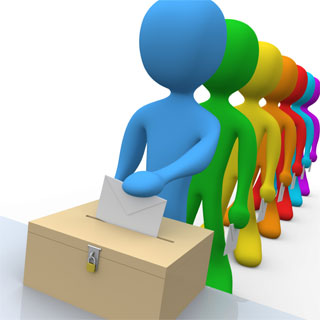
\includegraphics[scale=0.45]{copyrighted_image_01.jpeg} \\
    \textbf{Voting} \\
    Source: http://echrblog.blogspot.com/
  \end{center}
}

\frame{
  \frametitle{Example}

  \begin{center}
%    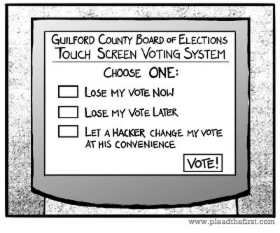
\includegraphics[scale=0.6]{copyrighted_image_02-01.jpg} \\
    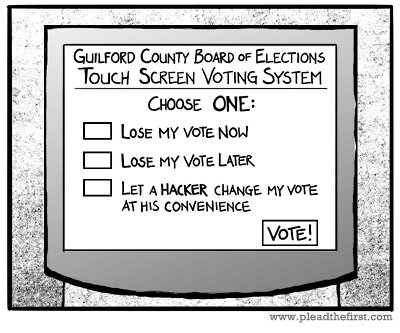
\includegraphics[scale=0.45]{copyrighted_image_02.jpg} \\
    \textbf{Wanna Vote for Yourself?} \\
    Source: http://pleadthefirst.com/
  \end{center}
}

\frame{
  \frametitle{Example}

  \begin{center}
    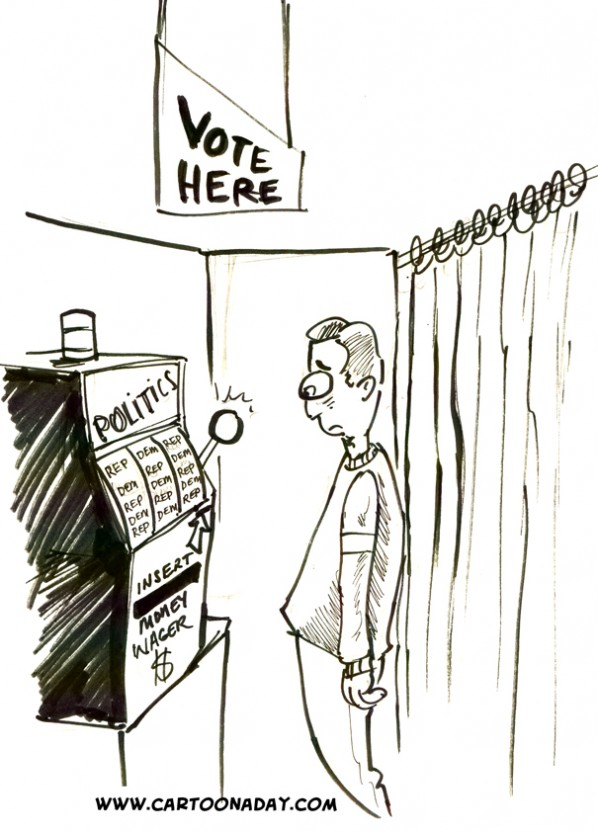
\includegraphics[scale=0.20]{copyrighted_image_03.jpg} \\
    \textbf{How Voting Should Work} \\
    Source: http://www.cartoonaday.com
  \end{center}
}

\section{Our Internet voting problem}

\frame{
  \begin{center}
    \textbf{\Huge{Our problem today}}
  \end{center}
}

\frame{
  \frametitle{Description}

  \begin{columns}[c]
    \column{2in}
    Given:

    \begin{itemize}
    \item name, and
    \item number of votes
    \end{itemize}

    for \textbf{a specified number} of candidates (\textbf{less than
      10} people).

    \column{2in}
    Find out the $1^{st}, 2^{nd},$ and the $3^{rd}$ winners.
  \end{columns}
}

\frame{
  \frametitle{Old story}

  \begin{center}
    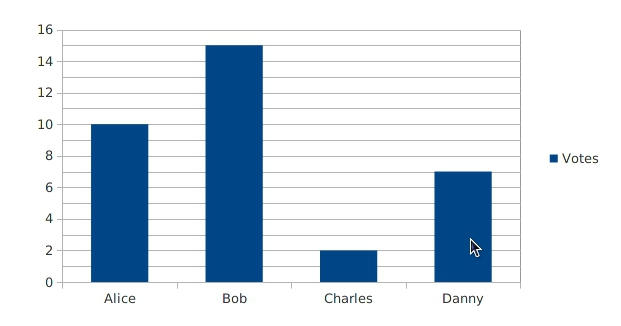
\includegraphics[scale=0.40]{chart_01.jpeg} \\
    Winners: \\
    \begin{itemize}
    \item<2-> $1^{st}$ place: Bob
    \item<2-> $2^{nd}$ place: Alice
    \item<2-> $3^{rd}$ place: Danny
    \end{itemize}
  \end{center}
}

\frame{
  \frametitle{Just 2 candidates}

  \begin{center}
    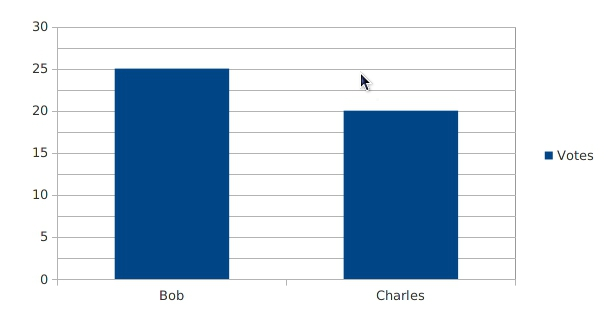
\includegraphics[scale=0.40]{chart_02_-_two_players_only.jpeg} \\
    Winners: \\
    \begin{itemize}
    \item<2-> $1^{st}$ place: Bob
    \item<2-> $2^{nd}$ place: Charles
    \item<2-> $3^{rd}$ place: (No one)
    \end{itemize}
  \end{center}
}

\frame{
  \frametitle{Tie}

  \begin{center}
    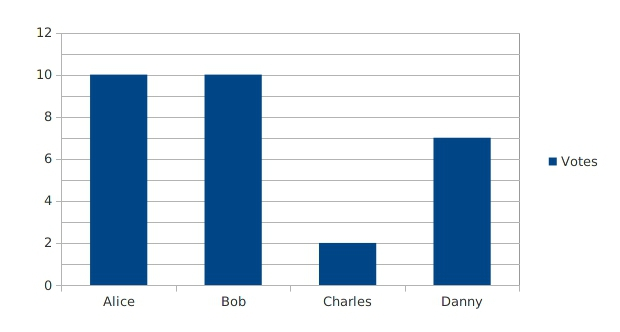
\includegraphics[scale=0.40]{chart_tie_01.jpeg} \\
    Winners: \\
    \begin{itemize}
    \item<2-> $1^{st}$ place: Alice, Bob
    \item<2-> $2^{nd}$ place: Danny
    \item<2-> $3^{rd}$ place: Charles
    \end{itemize}
  \end{center}
}

\frame{
  \frametitle{Tie, again}

  \begin{center}
    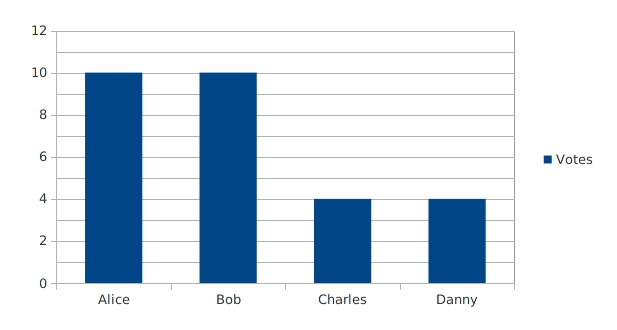
\includegraphics[scale=0.40]{chart_tie_02.jpeg} \\
    Winners: \\
    \begin{itemize}
    \item<2-> $1^{st}$ place: Alice, Bob
    \item<2-> $2^{nd}$ place: Charles, Danny
    \item<2-> $3^{rd}$ place: (No one)
    \end{itemize}
  \end{center}
}

\section{Solving with Randori}

\frame{
  \begin{center}
    \textbf{\Huge{Solving with Randori}}
  \end{center}
}

\frame{
  \begin{itemize}
    \item<1-> Writing tests first.
    \item<2-> Thinking (critically).
    \item<3-> Being a pilot/co-pilot and getting help.
    \item<4-> Don't forget to have fun!!!
  \end{itemize}
}

\frame{
  \begin{center}
    \textbf{\Huge Let's do it!!!}
  \end{center}
}

\frame{
  \begin{center}
    \textbf{\Huge Thank you for your attention!}
  \end{center}
}

\end{document}

%%% Local Variables: 
%%% mode: latex
%%% TeX-master: t
%%% End: 
